\documentclass{standalone}
\usepackage{tikz,amsmath,graphicx,calc,chemfig}
\usepackage[update,verbose=false]{epstopdf}
\usepackage[version=3]{mhchem}
\graphicspath{{./figs/}}
\usetikzlibrary{
    arrows,
    decorations.pathmorphing,
    shapes.geometric,
    backgrounds,
    positioning,
    fit,
    petri,
}
\setatomsep{1.4em}
\setbondoffset{.1em}
%\setcrambond{.3em}{1pt}{.0em}
\renewcommand*\printatom[1]{{\ensuremath{\mathsf{#1}}}}

\begin{document}
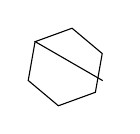
\begin{tikzpicture}
    [scale=1,
     structure/.style={rectangle,draw=white,fill=white,
               outer xsep=.2cm,outer ysep=.2cm,minimum size=2mm,node distance=0.4cm},
     label/.style={rectangle,fill=white,font=\bfseries,
               outer ysep=.2cm,minimum size=4mm,},
     arrow/.style={->,>=stealth',semithick},
     reagent/.style={text width=2cm,font=\footnotesize,align=center,midway},
     designbox/.style={rectangle,draw=black,thick,fill=red,
               inner sep=0pt,minimum width=15mm, minimum height=2.5mm, node distance=0mm},
               line join=miter]
    %
    \node [shape=regular polygon, regular polygon sides=6, minimum size=1cm, draw,rotate=260] (hexane) at (0,0) {};
    \draw [relative] (hexane.corner 4) --++ (-30:1) node{};
    
    
\end{tikzpicture}
\end{document}
